\section{Credit Capacity under Repayment Rights}\label{sec:credit}

\Cref{lem:exact} gives the cash needed for redemptions at one state. A lending rule must also cover the states that borrowers can create by repaying. This section characterizes that requirement for a fixed curve, and the next two sections draw its consequences: what a reserve committed to above-floor lending is exposed to, and what a different release rule can do without one.

\subsection{Repayment rights and cash coverage}\label{cr:rights}

Fix a schedule $p$ and its reserve function $R$. There are finitely many loans $(\ell_i,d_i)$, with $\ell_i,d_i>0$, total lock $L\le S$, and cash $A\ge0$. Custody holds, and $W=A+D-R(S)\ge0$. We allow debts above the floor, so (J2) is \emph{not} assumed. Initially consider only repayments and redemptions at their full gross curve return. There is no new borrowing, minting, reshaping, accrual, reserve withdrawal or fee retention. Thus $W$ is constant. Borrowers may supply the cash needed to repay; safety is required for all allowed repayment choices, whether or not those choices maximize their payoffs.

For each loan, let $\mathcal E_i\subseteq[0,\ell_i]\times[0,d_i]$ be the closure of the set of residual pairs $(q_i,b_i)$, locked tokens and remaining debt, attainable by a finite sequence of repayments. It includes the initial pair and $(0,0)$. Repayment rights are local to the loan: they do not depend on other loans, free balances or redemptions. Each combination of attainable pairs can therefore be reached by making the loans' repayments in turn, before any redemption. Taking the closure includes limits of such combinations; the cash inequalities below are continuous and are unchanged by this convention. Full repayment releases the whole lock. We call a state \emph{safe under its repayment rights} if every finite sequence of these repayments and gross redemptions can be executed without a cash shortfall.

\begin{theorem}[Coverage under repayment rights]\label{cr:kernel}
The state is safe under its repayment rights if and only if
\begin{equation}\label{cr:allpairs}
\sum_i b_i\;\le\;W+R\!\left(\sum_i q_i\right)
\qquad\text{for every }(q_i,b_i)\in\mathcal E_i\text{ for all }i.
\end{equation}
When $W=0$, this is equivalent to the separate conditions
\begin{equation}\label{cr:individual}
b\le R(q)\qquad\text{for every }(q,b)\in\mathcal E_i\text{ and every }i.
\end{equation}
\end{theorem}
\begin{proof}
After any repayments and redemptions, write $S',D',L',A'$ for the current state. Repayments preserve $A+D$, and a gross redemption reduces $A$ and $R(S)$ by the same amount. Thus $A'+D'-R(S')=W$. Redeeming all free tokens would leave cash
\[
A'-[R(S')-R(L')]=W+R(L')-D'.
\]
If \eqref{cr:allpairs} holds, that cash is non-negative at every possible loan state; every smaller redemption can also be paid. Repayments add cash. Conversely, a violation at an attainable residual configuration is exposed by making those repayments and then redeeming all free tokens. A strict violation at a limit configuration is also a violation at a nearby attainable one.

For the last claim, convexity and $R(0)=0$ give
\begin{equation}\label{cr:superadd}
\sum_i R(q_i)\le R\!\left(\sum_iq_i\right).
\end{equation}
Indeed $R(q_i)\le q_i R(Q)/Q$ for $Q=\sum_iq_i>0$. Hence \eqref{cr:individual} suffices. It is necessary because all loans other than $i$ can be fully repaid, leaving their residual pairs equal to $(0,0)$.
\end{proof}

For any repayment rights we write $W_{\min}$ for the least reserve that satisfies \eqref{cr:allpairs}: the supremum of $\sum_ib_i-R(\sum_iq_i)$ over attainable configurations, which is at least zero. \Cref{cr:buffer} computes it for proportional release.

The quantifier over future repayments is essential. For $R(q)=q+q^2/2$, a one-token lock against debt $3/2$ satisfies the current condition $D=R(L)$. If $S=L=1$ and $W=0$, cash is zero. Repaying $3/4$ and releasing half the collateral makes $3/4$ cash available, but redeeming the released half costs $R(1)-R(1/2)=7/8$. The shortfall is $1/8$. No price movement or other borrower is needed.

\subsection{Proportional release and the committed reserve}\label{cr:proportional}\label{sec:credit-buffer}

Under proportional release, $\mathcal E_i=\{(x\ell_i,xd_i):0\le x\le1\}$. Put $a_i=d_i/\ell_i$. For $0\le q\le L$, define
\begin{equation}\label{cr:envelope}
H(q)=\max\left\{\sum_i a_iq_i:
0\le q_i\le\ell_i,\ \sum_iq_i=q\right\}.
\end{equation}
This is the fractional-knapsack envelope: retain collateral from loans with the largest $a_i$ first \citep{kellerer2004}. It is continuous, concave and piecewise linear. For $L>0$, if $Z$ takes value $a_i$ with probability $\ell_i/L$, then $H(q)=L\int_{1-q/L}^{1}F_Z^{-1}(u)\,du$ with $F_Z^{-1}$ the quantile function of $Z$, an upper integrated-quantile function \citep{gushchin2017}. For an empty book, set $H(0)=W_{\min}=0$. The sorting argument is classical; its role here is to identify the residual loan book that places the greatest demand on cash.

\begin{theorem}[Exact buffer for proportional release]\label{cr:buffer}
With proportional release, the least non-negative committed reserve required by \cref{cr:kernel} is
\begin{equation}\label{cr:wmin}
W_{\min}=\max_{0\le q\le L}\{H(q)-R(q)\}.
\end{equation}
In particular, when $W=0$, safety under all repayment choices holds if and only if $d_i\le\Pf\ell_i$ for every loan. This necessity applies to heterogeneous and state-dependent loan allocations, not only to a uniform cap.
\end{theorem}
\begin{proof}
At fixed residual total $q$, \eqref{cr:envelope} is the largest possible remaining debt. Substitution in \cref{cr:kernel} gives \eqref{cr:wmin}; its maximum is at least zero because $H(0)=R(0)=0$. For $W=0$, \eqref{cr:individual} requires $xd_i\le R(x\ell_i)$ for every $x>0$. Divide by $x\ell_i$ and let $x$ decrease to zero to obtain $a_i\le\Pf$. Conversely, $a_iq_i\le\Pf q_i\le R(q_i)$, so \eqref{cr:individual} holds.
\end{proof}

For a uniform cap per token, the necessity of the floor bound is \cref{prop:tight}. The statement here extends it in two ways: it holds loan by loan for any allocation of debt, and it follows from the repayment rights alone, without constructing a sequence of borrowing operations.

The function $H-R$ is concave. Its maximum is found where the non-increasing slope of $H$ crosses the non-decreasing price $p$, including endpoints and jumps. Sorting the ratios takes $O(n\log n)$ comparisons. With rational stepped or piecewise-affine prices, a scan of the price and collateral breakpoints finds the maximum exactly. \Cref{cr:algorithm} gives the representation and algorithm; an arbitrary price function instead requires an evaluation or optimization oracle.

\paragraph{Keeping the reserve committed.}
For this extended design, $W$ is not all available for withdrawal. The safe skim guard is $w\le W-W_{\min}$. A repayment restricts the remaining possible residual configurations, so it cannot increase $W_{\min}$ at a fixed curve. Gross sales leave both $W$ and the loan book unchanged; retaining fees can only increase $W$. New lending may be admitted by checking $W'\ge W_{\min}'$ in the resulting state. That test also implies $A'\ge0$, since the initial residual configuration gives $D'\le W'+R(L')\le W'+R(S')$. A reshape needs the same test with the new reserve function and the repayment rights that will remain in force. These are guards for a different mechanism; the original \op{Skim} guard in \cref{sec:model} must not be used with above-floor proportional loans. Full derivations are in \cref{cr:guards}.

\subsection{Allocation of a fixed reserve}\label{cr:allocation}

\begin{proposition}[Equal ratios and aggregate capacity]\label{cr:capacity}
Fix positive lock sizes with total $L>0$. Among allocations with total debt $D$, assigning $d_i=(D/L)\ell_i$ minimizes $W_{\min}$, weakly. The greatest aggregate debt consistent with proportional release and a committed reserve $W\ge0$ is
\begin{equation}\label{cr:dmax}
D_{\max}=L\inf_{0<q\le L}\frac{R(q)+W}{q}.
\end{equation}
An allocation with equal ratios attains this bound.
\end{proposition}
\begin{proof}
Concavity, $H(0)=0$ and $H(L)=D$ imply $H(q)\ge Dq/L$. Equal ratios attain equality at every $q$, so they weakly minimize \eqref{cr:wmin}. For that allocation, the safety constraints are $(D/L)q\le R(q)+W$ for every $q>0$, which are equivalent to \eqref{cr:dmax}. The infimum is finite and the corresponding constant ratio satisfies every constraint, whether or not the infimum is attained at a positive $q$.
\end{proof}

The minimizer need not be unique. This is a chord comparison for the classical envelope, rather than a new general optimization method. Its implication for credit is that two books with identical supply and total debt can require different reserves. With $R(q)=q+q^2/2$, $L=1$ and $D=3/2$, an equal ratio of $3/2$ requires $W_{\min}=1/8$. Two locks of $1/2$ with debts $1$ and $1/2$ require $W_{\min}=3/8$: the highest ratio is retained while the other loan is repaid. The reserve requirement triples although aggregate utilization is unchanged.

\begin{figure}[t]
\centering
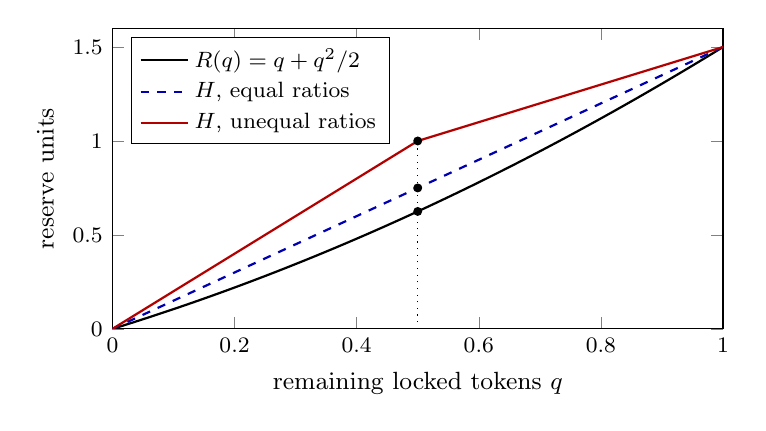
\begin{tikzpicture}
\begin{axis}[width=0.77\textwidth,height=5.4cm,
  xlabel={remaining locked tokens $q$},ylabel={reserve units},
  xmin=0,xmax=1,ymin=0,ymax=1.6,
  legend pos=north west,legend cell align=left,
  tick label style={font=\footnotesize},label style={font=\small},
  legend style={font=\footnotesize}]
\addplot[thick,black,domain=0:1,samples=101] {x+x*x/2};
\addlegendentry{$R(q)=q+q^2/2$}
\addplot[thick,dashed,blue!70!black,domain=0:1,samples=2] {1.5*x};
\addlegendentry{$H$, equal ratios}
\addplot[thick,red!70!black] coordinates {(0,0) (0.5,1) (1,1.5)};
\addlegendentry{$H$, unequal ratios}
\draw[thin,dotted] (axis cs:0.5,0) -- (axis cs:0.5,1);
\addplot[only marks,mark=*,mark size=1.4pt,black]
  coordinates {(0.5,0.625) (0.5,0.75) (0.5,1)};
\end{axis}
\end{tikzpicture}
\caption{The required reserve is the greatest vertical distance from $R$ to the debt envelope $H$. Both books have $L=1$ and $D=3/2$. Their maximum gaps occur at $q=1/2$ and are $1/8$ for equal ratios and $3/8$ for the two unequal ratios. These quantities are checked in script block CF01.}\label{cr:figure}
\end{figure}

For the linear price $p(q)=P+kq$, with $P>0$ and $k>0$, minimizing \eqref{cr:dmax} gives
\begin{equation}\label{cr:linearcapacity}
\frac{D_{\max}}L=
\begin{cases}
P, & W=0,\\[2pt]
P+\sqrt{2kW}, & 0<W\le kL^2/2,\\[2pt]
P+kL/2+W/L, & W>kL^2/2.
\end{cases}
\end{equation}
The interior minimizing depth is $\sqrt{2W/k}$. The formula describes cash coverage, not a positive residual for every borrower. An above-floor proportional loan can become worth less than its debt after a partial repayment, even when the committed reserve makes every free redemption payable. For example, in the one-token case above, $W=1/8$ pays the released half, but the remaining debt $3/4$ exceeds $R(1/2)=5/8$. A collateral-funded close is a separate requirement.

